%=====================================================================
\chapter{Multi-Source Data Integration Framework}
\label{ch:fusion}
%=====================================================================

\textbf{Research Objective 1.} \emph{To investigate and develop a comprehensive model that
integrates diverse data sources --- such as financial metrics, news articles, social media
sentiment and macroeconomic factors --- aiming to enhance the accuracy of stock market
predictions by providing a holistic analysis.}

\vspace{0.4em}
This chapter develops the first component of the thesis: a hierarchical architecture that
integrates four heterogeneous streams of Indian market information and produces a forecast whose
improvement over simpler alternatives can be \emph{attributed} to identifiable causes rather
than merely observed. Section~\ref{sec:msfn-arch} specifies the architecture,
Section~\ref{sec:msfn-data} the data and the alignment protocol, Section~\ref{sec:msfn-setup}
the experimental design and its assumptions, and Sections~\ref{sec:msfn-results}
to~\ref{sec:msfn-robust} the evidence. Section~\ref{sec:msfn-limits} states what the chapter does
not establish, which is what motivates Chapter~\ref{ch:dynfusion}.

The work reported in this chapter appears in publication~\pubcite{P1}.

\section{Design Rationale}
\label{sec:msfn-rationale}

Three design decisions distinguish the Multi-Source Fusion Network from the fusion
architectures reviewed in Section~3.1, and each is a response to a limitation identified there.

\textbf{Modality-specific encoding before cross-modal combination.} Early fusion concatenates
raw features from every source and asks a single architecture to learn both within-domain and
cross-domain structure. That is inefficient and prone to modality dominance: a stream with many
features or large numerical magnitudes crowds out one with few. The architecture developed here
learns a representation \emph{within} each modality first, using an encoder matched to that
modality's structure, and combines only the learned representations. Each stream is therefore
encoded in the form appropriate to it --- convolution over indicator sequences, transformer
encoding over text, engineered temporal features over slow macroeconomic series --- before any
cross-modal interaction occurs.

\textbf{Time-varying rather than fixed source weighting.} The combination is performed by
cross-modal attention, with relevance weights recomputed at every time step rather than fixed by
the architecture. This is what allows the model to express the proposition that news mattered
more than price history on a particular day. Section~\ref{sec:msfn-attention} examines the
learned distribution and shows that it is genuinely state-dependent rather than approximately
constant, which is the empirical justification for the mechanism.

\textbf{Attributability as a design requirement.} The architecture is constructed so that each
stream can be removed and the model retrained without changing anything else. This is not free:
it constrains the encoders to be modular and prevents certain forms of parameter sharing. The
return on that constraint is Section~\ref{sec:msfn-ablation}, which reports the marginal value
of each stream rather than asserting that all of them help.

\section{Architecture of the Multi-Source Fusion Network}
\label{sec:msfn-arch}

The architecture is organised as five layers, shown in Figure~\ref{fig:msfn}: acquisition,
preprocessing, feature extraction, fusion and prediction.

\begin{figure}[!htb]
\centering
\scalebox{0.88}{\begin{tikzpicture}[node distance=3mm]
\node[blkd,minimum width=25mm,minimum height=8mm] (d1) {Financial data\\NSE / BSE};
\node[blkd,right=3mm of d1,minimum width=25mm,minimum height=8mm] (d2) {News articles\\financial press};
\node[blkd,right=3mm of d2,minimum width=25mm,minimum height=8mm] (d3) {Social media\\X, StockTwits};
\node[blkd,right=3mm of d3,minimum width=25mm,minimum height=8mm] (d4) {Macro data\\RBI, MOSPI, IMF};

\node[blk,below=6mm of d1,minimum width=25mm,minimum height=8mm] (p1) {15 technical\\indicators};
\node[blk,below=6mm of d2,minimum width=25mm,minimum height=8mm] (p2) {Transformer\\sentiment scoring};
\node[blk,below=6mm of d3,minimum width=25mm,minimum height=8mm] (p3) {Lexicon + LSTM\\sentiment scoring};
\node[blk,below=6mm of d4,minimum width=25mm,minimum height=8mm] (p4) {Normalisation and\\daily interpolation};

\node[blkg,below=6mm of p1,minimum width=25mm,minimum height=8mm] (e1) {CNN\\feature maps};
\node[blkg,below=6mm of p2,minimum width=25mm,minimum height=8mm] (e2) {Text\\embeddings};
\node[blkg,below=6mm of p3,minimum width=25mm,minimum height=8mm] (e3) {Text\\embeddings};
\node[blkg,below=6mm of p4,minimum width=25mm,minimum height=8mm] (e4) {Temporal\\features};

\node[blka,below=7mm of e2,minimum width=79mm,minimum height=8mm,xshift=14mm] (att)
  {Cross-modal attention $\;\to\;$ concatenation $\;\to\;$ adaptive weighting};
\node[blka,below=5mm of att,minimum width=79mm,minimum height=8mm] (bl)
  {Bi-LSTM encoder with temporal attention $\;\to\;$ dense layers with dropout};
\node[blkd,below=5mm of bl,minimum width=79mm,minimum height=7mm] (o)
  {Predicted level and direction with confidence interval, horizon $\tau \in \{1,3,7,15\}$ days};

\foreach \a/\b in {d1/p1,d2/p2,d3/p3,d4/p4,p1/e1,p2/e2,p3/e3,p4/e4}
  \draw[ar] (\a) -- (\b);
\foreach \a in {e1,e2,e3,e4} \draw[ar] (\a.south) -- ++(0,-2mm) -| (att.north);
\draw[ar] (att) -- (bl);
\draw[ar] (bl) -- (o);
\node[lbl,rotate=90,anchor=center,align=center]
  at ([xshift=-8mm]$(d1.west)!0.5!(p1.west)$) {acquisition};
\node[lbl,rotate=90,anchor=center,align=center]
  at ([xshift=-8mm]$(p1.west)!0.5!(e1.west)$) {preprocessing and\\feature extraction};
\node[lbl,rotate=90,anchor=center] at ([xshift=-8mm]d1.west |- att) {fusion};
\node[lbl,rotate=90,anchor=center] at ([xshift=-8mm]d1.west |- o) {prediction};
\end{tikzpicture}}
\caption[Architecture of the Multi-Source Fusion Network]{Architecture of the Multi-Source
Fusion Network, showing the flow from heterogeneous acquisition through modality-specific
preprocessing and feature extraction to cross-modal fusion and prediction.}
\label{fig:msfn}
\end{figure}

\subsection{Acquisition and preprocessing}

The acquisition layer collects raw inputs from four interfaces: exchange price and volume
records, financial press feeds, social media platforms, and official macroeconomic
publications. The preprocessing layer standardises them. Technical indicators are computed from
closing series; news and social text are scored; macroeconomic series are normalised and aligned
to a daily frequency. Section~\ref{sec:msfn-data} gives the detail and states the cost of each
alignment decision.

\subsection{Modality-specific encoders}

Each preprocessed modality $m$ is passed through a stack of one-dimensional convolutional
layers,
\begin{equation}
h_m^{(l)} = \mathrm{ReLU}\!\left(\mathrm{Conv1D}\!\left(W_m^{(l)} * h_m^{(l-1)} +
b_m^{(l)}\right)\right),
\label{eq:msfn-conv}
\end{equation}
where $h_m^{(0)}$ is the raw feature matrix of modality $m$, $W_m^{(l)}$ and $b_m^{(l)}$ are the
learnable convolution kernel and bias at layer $l$, $*$ denotes convolution along the time axis,
and max-pooling follows each convolutional block. Convolution is appropriate for indicator
streams because the patterns of interest --- a crossover, a band squeeze, a volume spike --- are
local and translation-invariant in time. For the two textual modalities the same notation
applies to the sequence of daily aggregated scores; the contextual reading of individual
documents has already been performed by the sentiment encoders described in
Section~\ref{sec:msfn-data}.

\subsection{Cross-modal attention}

The fusion layer computes a relevance weight for each modality by scaled dot-product attention
over the modality representations,
\begin{equation}
\alpha_m = \mathrm{softmax}\!\left(\frac{q \cdot k_m}{\sqrt{d_k}}\right),
\label{eq:msfn-attn}
\end{equation}
where $q$ is a query vector learned during training, $k_m$ is the key vector of modality $m$ and
$d_k$ is the key dimension. The fused representation at session $t$ is the attention-weighted
combination of the modality representations,
$F_t = \sum_m \alpha_m^{(t)}\, h_m^{(L)}(t)$, followed by concatenation with the unweighted
representations so that no modality can be suppressed entirely by a degenerate attention
distribution.

The essential property is that $\alpha_m$ is recomputed at every time step. A fixed-weight
scheme --- whether a hand-set constant or a single set of learned coefficients --- asserts that
the relative informativeness of price history and news is the same in a calm trending market as
during an earnings announcement. Equation~\eqref{eq:msfn-attn} does not make that assertion, and
Section~\ref{sec:msfn-attention} shows that the data do not support it.

\subsection{Temporal modelling and output}

The fused representation is passed through two bidirectional recurrent layers,
\begin{align}
\overrightarrow{h}_t &= \mathrm{LSTM}(F_t, \overrightarrow{h}_{t-1}), &
\overleftarrow{h}_t &= \mathrm{LSTM}(F_t, \overleftarrow{h}_{t+1}), &
h_t &= [\overrightarrow{h}_t ; \overleftarrow{h}_t],
\label{eq:msfn-bilstm}
\end{align}
with a temporal attention layer over the hidden sequence, and the forecast is produced by dense
layers with dropout,
\begin{equation}
\hat{y}_{t+\tau} = W_o \cdot \mathrm{Dropout}(h_t) + b_o,
\qquad \tau \in \{1, 3, 7, 15\}\ \text{days}.
\label{eq:msfn-out}
\end{equation}
The backward pass in Equation~\eqref{eq:msfn-bilstm} reads the input window in reverse; this is
context \emph{within} the supplied window, which closes at the decision time, and is therefore
not look-ahead. Confidence intervals are produced from the dispersion of the dense-layer output
under repeated dropout sampling.

\section{Data, Sources and Temporal Alignment}
\label{sec:msfn-data}

\subsection{Study universe and period}

The study covers January 2015 to December 2024 --- ten years, spanning demonetisation, the
introduction of the goods and services tax, the COVID-19 crash and recovery, and the
inflation-driven repricing of 2022 --- on the NIFTY~50 index and ten sectoral indices:
financials, information technology, pharmaceuticals, energy, fast-moving consumer goods,
automobiles, metals, real estate, consumer durables and healthcare. Index-level data are used
rather than single names, which removes survivorship bias by construction, although composition
drift through constituent revisions remains.

Table~\ref{tab:msfn-data} records the four streams, their sources, frequencies and extracted
attributes.

\begin{table}[!htb]
\centering
\caption[Multi-source data characteristics for the Indian market study]{Multi-source data
characteristics for the Indian market study, January 2015 to December 2024}
\label{tab:msfn-data}
\tabfont
\begin{tabular}{@{}L{2.5cm}L{3.7cm}L{2.2cm}L{5.4cm}@{}}
\toprule
\textbf{Category} & \textbf{Source} & \textbf{Frequency} & \textbf{Attributes extracted} \\
\midrule
Financial metrics & NSE interfaces, Yahoo Finance & Daily & Open, high, low, close, volume;
fifteen derived technical indicators covering trend, momentum, volatility and participation \\
News articles & Economic Times, Moneycontrol, Bloomberg Quint & Real time & Headline and body
text, publication time stamp, source authority weight, computed polarity \\
Social media & X (formerly Twitter), StockTwits & Real time & Post text, engagement counts,
author following; daily aggregate polarity, mention volume, sentiment dispersion \\
Macroeconomic & RBI Bulletin, MOSPI, IMF & Monthly / quarterly & GDP growth, CPI and WPI
inflation, repo rate, index of industrial production, crude oil price \\
\bottomrule
\end{tabular}
\end{table}

\subsection{Feature engineering by modality}

\textbf{Financial metrics.} Fifteen technical indicators are derived from the price and volume
record, following the definitions in Section~2.2: moving averages over 5, 10 and 20 sessions and
the slope of the exponential average for trend; the relative strength index and the moving
average convergence divergence with its signal line for momentum; Bollinger band width and
position, average true range and realised volatility for volatility; and on-balance volume,
volume-weighted average price derivatives and volume momentum for participation.

\textbf{News sentiment.} Financial news is scored by a domain-adapted transformer encoder of the
FinBERT family~\cite{araci2019}. For each trading session the scores of all articles referencing
the target index or sector are aggregated, weighted by relevance to the instrument and by an
authority weight attached to the source. Domain adaptation matters here for the reason Loughran
and McDonald~\cite{loughran2011} identified: a general-purpose model reads ``provision'' and
``liability'' as negative in text where they are neutral accounting vocabulary.

\textbf{Social media sentiment.} Posts from X and StockTwits are scored by a hybrid model
combining the VADER lexicon~\cite{hutto2014}, which handles the intensifiers, negations and
orthographic emphasis characteristic of social text, with a recurrent classifier fine-tuned on
financial social media. Three daily aggregates are retained: mean polarity, mention volume and
sentiment dispersion. Dispersion is included deliberately: a day on which opinion is uniformly
positive carries different information from one on which the mean is the same but opinion is
split, and it also serves as a partial diagnostic for coordinated posting.

\textbf{Macroeconomic indicators.} Six series are used: GDP growth, consumer price and wholesale
price inflation, the RBI repo rate, the index of industrial production, and crude oil prices,
obtained from RBI bulletins and official statistics. The series are normalised and interpolated
to daily frequency.

\subsection{Temporal alignment and its costs}

Every stream is aligned to the NSE trading calendar under the four rules of Section~2.5. Two
alignment decisions introduce distortions that are stated here rather than left implicit,
because they bound the interpretation of the results.

The first is macroeconomic interpolation. Monthly and quarterly series are interpolated to daily
frequency, which assumes that information flows smoothly between releases. It does not:
macroeconomic effects are concentrated on announcement days. The direction of the resulting bias
is known --- interpolation \emph{understates} short-horizon announcement-day effects --- so the
macroeconomic contribution measured in Section~\ref{sec:msfn-ablation} should be read as a lower
bound on the contribution an event-aware treatment would find.

The second is daily aggregation of text. Aggregating news and social posts to a daily score
discards the ordering of items within the day, trading microstructure detail for tractability.
At a daily decision horizon this is an acceptable trade, but it means the framework cannot
express the difference between a positive headline that preceded a negative one and the reverse.

\section{Experimental Setup}
\label{sec:msfn-setup}

\subsection{Partitioning and leakage control}

The data are partitioned chronologically into three contiguous blocks: training from January
2015 to December 2021 (70 per cent), validation from January 2022 to June 2023 (15 per cent),
and test from July 2023 to December 2024 (15 per cent). All features are standardised to zero
mean and unit variance using \emph{training-set statistics only}. Hyperparameters are selected on
the validation block and the test block is examined once, after the configuration is fixed.

\subsection{Hyperparameter selection}

Hyperparameters were tuned by grid search on the validation block over learning rates
$\{10^{-2}, 10^{-3}, 10^{-4}\}$, recurrent hidden sizes $\{64, 128, 256\}$, convolutional filter
counts $\{32, 64, 128\}$, dropout rates $\{0.2, 0.3, 0.5\}$ and batch sizes $\{32, 64, 128\}$.
The selected configuration is reported in Table~\ref{tab:msfn-hyper}.

\begin{table}[!htb]
\centering
\caption[Selected architecture and training configuration]{Selected architecture and training
configuration for the Multi-Source Fusion Network}
\label{tab:msfn-hyper}
\tabfont
\begin{tabular}{@{}L{5.0cm}L{4.2cm}L{4.6cm}@{}}
\toprule
\textbf{Component} & \textbf{Setting} & \textbf{Selection basis} \\
\midrule
Convolutional encoder & 64 filters, kernel size 3, max-pooling & Validation loss; larger filter
counts did not improve validation error \\
Recurrent encoder & Two bidirectional layers, 128 hidden units & Validation loss; 256 units
over-fitted within the patience window \\
Dropout & 0.3 on dense layers & Validation loss \\
Optimiser & Adam, learning rate $10^{-3}$~\cite{kingma2015adam} & Grid search \\
Batch size & 64 & Grid search \\
Early stopping & Patience 10 epochs on validation loss & Fixed \emph{a priori} \\
Trainable parameters & $\approx 2.1$ million, majority in the recurrent layers & --- \\
Training time & Under two hours on a single consumer-grade accelerator & --- \\
Inference latency & Milliseconds per forward pass & --- \\
\bottomrule
\end{tabular}
\end{table}

Random seeds for data shuffling and weight initialisation were fixed across all runs, and an
identical preprocessing pipeline was applied to every model variant, so that reported
comparisons reflect architectural differences alone rather than initialisation noise.

\subsection{Baselines}

Six baselines are used, chosen so that the comparison isolates specific claims rather than
merely demonstrating that the proposed model wins.

\begin{itemize}
\item \textbf{ARIMA}, the classical statistical reference, establishing what linear time-series
structure alone achieves.
\item \textbf{LSTM (price only)} and \textbf{Transformer (price only)}, establishing the ceiling
for a single-source deep model.
\item \textbf{LSTM + sentiment} and \textbf{LSTM + macro}, establishing the incremental value of
each added stream under a simple architecture.
\item \textbf{Simple-average ensemble}, combining the single-source models with fixed equal
weights. This is the critical baseline: it consumes \emph{exactly the same four sources} as the
proposed model, so any difference between the two isolates the fusion mechanism from the data.
\end{itemize}

\subsection{Experimental assumptions}

Four assumptions are embedded in the evaluation and are recorded with their consequences.
First, macroeconomic interpolation understates announcement-day effects, as discussed above.
Second, daily sentiment aggregation discards within-day ordering. Third, the evaluation assumes
frictionless markets: transaction costs, slippage and market impact are not modelled, so
directional accuracy does not translate directly into trading profit --- a point taken up
seriously in Chapter~\ref{ch:allocation}, where costs are charged. Fourth, relationships learned
in the training window are assumed to hold in the test window; structural breaks would violate
this, which is precisely why the walk-forward analysis of Section~\ref{sec:msfn-robust} was
conducted.

\section{Results: Prediction Performance}
\label{sec:msfn-results}

Table~\ref{tab:msfn} reports one-day-ahead prediction on the NIFTY~50 index against the six
baselines, together with the source ablation that is discussed in
Section~\ref{sec:msfn-ablation}. The two blocks are presented as a single table because the two
questions they answer --- does fusion help, and which source is responsible --- are answered by
the same experiment.

\begin{table}[!htb]
\centering
\caption[Prediction performance and source ablation on the NIFTY 50 index]{One-day-ahead
prediction on the NIFTY~50 index: comparison against baselines (upper block) and source ablation
of the proposed model (lower block)}
\label{tab:msfn}
\tabfont
\begin{tabular}{@{}L{4.8cm}L{3.4cm}rrrr@{}}
\toprule
\textbf{Configuration} & \textbf{Data sources} & \textbf{MAE} & \textbf{RMSE} &
\textbf{$R^2$} & \textbf{DA (\%)} \\
\midrule
\multicolumn{6}{@{}l@{}}{\textit{Baseline comparison}}\\
ARIMA & price only & 0.124 & 0.167 & 0.721 & 52.3 \\
LSTM & price only & 0.087 & 0.112 & 0.845 & 61.7 \\
Transformer & price only & 0.079 & 0.103 & 0.869 & 64.2 \\
LSTM + sentiment & price, sentiment & 0.052 & 0.071 & 0.921 & 72.8 \\
LSTM + macro & price, macro & 0.061 & 0.082 & 0.903 & 68.5 \\
Ensemble (simple average) & all, fixed weights & 0.043 & 0.059 & 0.942 & 76.3 \\
\textbf{MSFN (proposed)} & \textbf{all, adaptive fusion} & \textbf{0.018} &
\textbf{0.024} & \textbf{0.988} & \textbf{84.7} \\
\midrule
\multicolumn{6}{@{}l@{}}{\textit{Source ablation of the proposed model}}\\
$-$ financial metrics & news, social, macro & 0.041 & 0.055 & 0.946 & 73.2 \\
$-$ news sentiment & price, social, macro & 0.027 & 0.036 & 0.971 & 79.1 \\
$-$ social media & price, news, macro & 0.025 & 0.033 & 0.976 & 80.8 \\
$-$ macroeconomic & price, news, social & 0.031 & 0.040 & 0.965 & 76.5 \\
$-$ both sentiment sources & price, macro & 0.038 & 0.049 & 0.952 & 74.0 \\
price and technical only & price only & 0.079 & 0.103 & 0.869 & 64.2 \\
\bottomrule
\end{tabular}
\end{table}

Three readings follow from the upper block.

\textbf{Deep architectures beat linear structure, but not decisively.} The price-only recurrent
model improves on ARIMA from a mean absolute error of 0.124 to 0.087 and from 52.3 to 61.7 per
cent directional accuracy; the price-only transformer improves further to 0.079 and 64.2 per
cent. The gain is real and it is bounded: a better architecture on the same information buys
roughly twelve percentage points of directional accuracy over a linear model and then
plateaus.

\textbf{Additional sources beat better architectures on the same source.} Adding sentiment to a
plain recurrent model raises directional accuracy to 72.8 per cent --- a larger gain than
replacing the recurrent model with a transformer on price alone. The ordering is informative:
information is scarcer than modelling capacity in this problem.

\textbf{The fusion mechanism, not the data, produces the headline result.} The decisive
comparison is between the proposed model and the simple-average ensemble, because the two consume
identical inputs. The ensemble attains a mean absolute error of 0.043 and 76.3 per cent
directional accuracy; the proposed model attains 0.018 and 84.7 per cent. Since the data are
held constant, the difference is attributable to how the sources are combined. This is the
central claim of the chapter, and it is the reason the ensemble baseline was constructed.

\section{Source Contribution: Ablation}
\label{sec:msfn-ablation}

The lower block of Table~\ref{tab:msfn} removes one stream at a time and retrains.
Figure~\ref{fig:source-ablation} presents the degradations directly.

\begin{figure}[!htb]
\centering
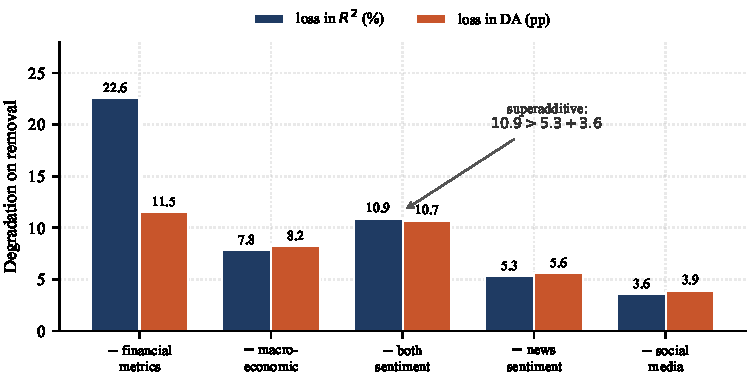
\includegraphics[width=0.86\linewidth]{figs/f_source_ablation.pdf}
\caption[Marginal cost of removing each source]{Marginal cost of removing each source from the
fused model, measured as the loss in explained variance and in directional accuracy. The joint
removal of both textual sources costs more than the sum of their individual removals.}
\label{fig:source-ablation}
\end{figure}

\textbf{Financial metrics are foundational but not sufficient.} Their removal is the single most
damaging ablation, costing 22.6 per cent of explained variance. This is the expected result and
would be worrying if it were otherwise. The complementary observation is more interesting:
restricting the model to price and technical features alone costs 32.0 percentage points of
directional accuracy relative to the full model, so the numerical stream is necessary and a long
way from sufficient.

\textbf{Macroeconomic indicators carry substantial weight.} Their removal costs 7.8 per cent of
explained variance. Given that interpolation understates announcement-day effects, this is a
lower bound. It is consistent with the structural observation of Section~2.1.2 that Indian equity
valuations are strongly sensitive to policy rates, inflation and industrial output.

\textbf{The two textual sources are complementary, not redundant.} This is the most informative
result in the table. Removing news sentiment alone costs 5.3 per cent of explained variance;
removing social media alone costs 3.6 per cent; removing both costs 10.9 per cent. Since
$10.9 > 5.3 + 3.6 = 8.9$, the joint effect exceeds the sum of the individual effects. That
superadditivity is the quantitative signature of complementary information: each textual source
partially covers for the other's absence, so removing one is cheap and removing both is
expensive. It is also the empirical justification for a fusion architecture rather than a larger
single-source model --- a model with more capacity on price data alone cannot recover information
that is not in the price data.

The finding is consistent with Fu and Zhang~\cite{fu2024}, who report that news sentiment supplies
the more stable signal and social media the more frequent directional one. Two streams that
differ in that way should be expected to substitute imperfectly for one another, which is exactly
what the superadditivity measures.

\section{Where the Gain Comes From: Attention Analysis}
\label{sec:msfn-attention}

The ablation establishes that all four sources contribute. The attention distribution establishes
\emph{when} each contributes. Figure~\ref{fig:att} reports the learned weights under three market
conditions.

\begin{figure}[!htb]
\centering

\includegraphics[width=0.80\linewidth]{figs/f_attention.pdf}
\caption[Cross-modal attention weights by market regime]{Cross-modal attention weights learned
for each source under three market conditions. Source importance is state-dependent, which is the
property that fixed-weight fusion cannot represent.}
\label{fig:att}
\end{figure}

Averaged over the whole sample, financial metrics carry the highest weight at 35 per cent,
macroeconomic indicators 25 per cent, news sentiment 22 per cent and social media 18 per cent ---
so the two textual sources jointly account for 40 per cent of the attention mass. The averages
are not the finding. The finding is that the shares move:

\begin{itemize}
\item During \textbf{earnings season}, the financial metrics share rises from 35 to 42 per cent
and news sentiment from 22 to 28 per cent, while social media falls from 18 to 15 per cent and
macroeconomic indicators from 25 to 15 per cent. Company-specific numerical disclosure and the
reporting around it dominate; slow macroeconomic conditions matter less when a concrete earnings
number has just arrived.
\item Under \textbf{high volatility}, the pattern inverts. Financial metrics fall from 35 to 28
per cent and social media rises from 18 to 28 per cent. Technical patterns break down in
disturbed markets precisely when retail sentiment is most active and most influential.
\end{itemize}

The second pattern is independently corroborated. Khan and Chahal~\cite{khan2025asymmetric} find,
using a quantile-on-quantile approach on eleven Indian sectoral indices, that the influence of
social media sentiment on sectoral returns is strongest at market extremes. The attention
mechanism recovers that structure from the data without being told to look for it, which is
evidence that the learned weights are tracking something real rather than fitting noise.

This behaviour is what a fixed-weight scheme cannot reproduce, and it explains the margin over
the simple-average ensemble in Table~\ref{tab:msfn}. An ensemble that weights social media at 18
per cent at all times is materially misweighted in exactly the volatile periods where forecasting
errors are most costly.

\section{Sectoral Analysis}
\label{sec:msfn-sector}

Table~\ref{tab:msfn-sector} and Figure~\ref{fig:sector} report performance across the ten
sectoral indices.

\begin{table}[!htb]
\centering
\caption[Sector-wise prediction performance]{Sector-wise one-day-ahead prediction performance and
the dominant information channel in each sector}
\label{tab:msfn-sector}
\tabfont
\begin{tabular}{@{}L{2.6cm}rrrrL{4.8cm}@{}}
\toprule
\textbf{Sector} & \textbf{MAE} & \textbf{RMSE} & \textbf{$R^2$} & \textbf{DA (\%)} &
\textbf{Dominant information channel} \\
\midrule
Financials & 0.016 & 0.022 & 0.991 & 86.2 & RBI policy, credit growth \\
FMCG & 0.019 & 0.025 & 0.986 & 84.0 & Rural demand, inflation \\
IT & 0.021 & 0.028 & 0.982 & 82.5 & Global technology demand, USD/INR \\
Healthcare & 0.023 & 0.030 & 0.978 & 80.5 & Policy, public-health news \\
Pharmaceuticals & 0.024 & 0.031 & 0.976 & 80.1 & Regulatory news, USFDA actions \\
Automobiles & 0.026 & 0.034 & 0.972 & 78.9 & Interest rates, fuel prices \\
Consumer durables & 0.027 & 0.036 & 0.970 & 78.1 & Consumer credit \\
Energy & 0.029 & 0.037 & 0.968 & 77.3 & Crude oil, government policy \\
Metals & 0.032 & 0.041 & 0.961 & 75.2 & Global commodity prices \\
Real estate & 0.035 & 0.044 & 0.957 & 73.8 & Interest rates, housing demand \\
\bottomrule
\end{tabular}
\end{table}

\begin{figure}[!htb]
\centering
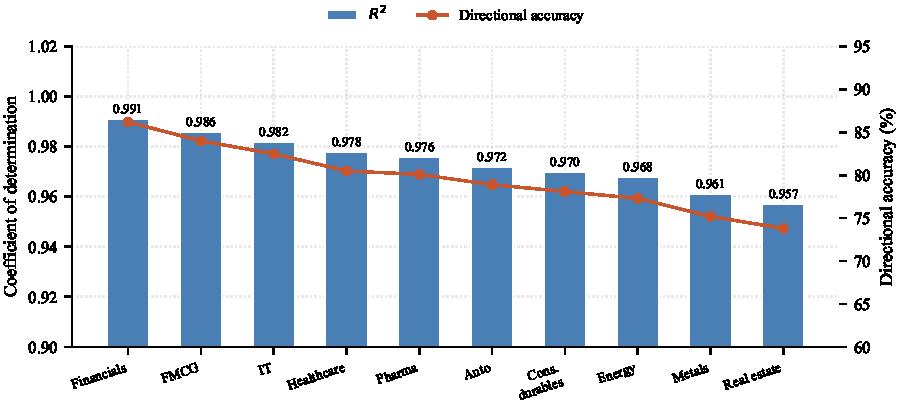
\includegraphics[width=0.92\linewidth]{figs/f_sector.pdf}
\caption[Sector-wise prediction quality]{Sector-wise prediction quality across ten NSE sectoral
indices. Predictability declines monotonically with exposure to exogenous global factors and with
the volatility of the sector.}
\label{fig:sector}
\end{figure}

Predictability varies by roughly three percentage points of explained variance and twelve
percentage points of directional accuracy between the most and least predictable sectors. The
ranking itself is of limited interest; its explanation is not. Two structural patterns are
visible.

The first is that predictability declines with exposure to factors exogenous to the domestic
information set. Financials and fast-moving consumer goods, whose drivers --- policy rates,
credit growth, rural demand, domestic inflation --- are all observable in the four streams,
attain $R^2$ above 0.985. Metals and real estate, whose drivers include global commodity prices
and construction-sector credit conditions that the framework observes only indirectly, fall
below 0.962.

The second is that the \emph{composition} of the contribution varies by sector. Sentiment
components contribute most in the globally exposed information technology and pharmaceutical
sectors, where regulatory announcements and demand commentary from overseas markets arrive first
as text; energy and metals depend more heavily on the macroeconomic stream, particularly global
commodity prices. Source importance is therefore structured by sector as well as by market
state, which strengthens the case for adaptive rather than fixed weighting: the appropriate
weight vector differs across both dimensions.

\section{Robustness: Walk-Forward Validation}
\label{sec:msfn-robust}

A directional accuracy of 84.7 per cent is high enough that the possibility of a split-induced
artefact must be addressed directly rather than argued away. The test period was therefore
divided into five sequential, non-overlapping folds, evaluated under an expanding-window
protocol in which each fold is scored only on sessions strictly later than its training window.
Table~\ref{tab:msfn-wf} and Figure~\ref{fig:wf} report the outcome.

\begin{table}[!htb]
\centering
\caption[Expanding-window walk-forward validation]{Expanding-window walk-forward validation over
the test period. Errors are normalised by the mean index level within each fold.}
\label{tab:msfn-wf}
\tabfont
\begin{tabular}{@{}lrrrr@{}}
\toprule
\textbf{Fold} & \textbf{MAE} & \textbf{RMSE} & \textbf{$R^2$} & \textbf{DA (\%)} \\
\midrule
1 & 0.0012 & 0.0014 & 0.881 & 80.0 \\
2 & 0.0014 & 0.0017 & 0.826 & 80.0 \\
3 & 0.0024 & 0.0032 & 0.868 & 92.0 \\
4 & 0.0016 & 0.0024 & 0.833 & 68.0 \\
5 & 0.0015 & 0.0018 & 0.960 & 72.0 \\
\midrule
\textbf{Mean} & \textbf{0.0016} & \textbf{0.0021} & \textbf{0.874} & \textbf{78.4} \\
Standard deviation & 0.0004 & 0.0006 & 0.048 & 8.2 \\
\bottomrule
\end{tabular}
\end{table}

\begin{figure}[!htb]
\centering

\includegraphics[width=0.98\linewidth]{figs/f_walkforward.pdf}
\caption[Expanding-window walk-forward validation and fold stability]{Expanding-window
walk-forward validation. (a) Protocol: each fold is evaluated only on sessions strictly later
than its training window. (b) Fold-wise directional accuracy and normalised mean absolute error
over the test period.}
\label{fig:wf}
\end{figure}

Three observations follow. The normalised errors are tightly clustered at
$0.0016 \pm 0.0004$, a coefficient of variation of about one quarter across folds separated in
time. Directional accuracy remains well above chance in every fold, ranging from 68 to 92 per
cent with a mean of 78.4 per cent; no fold approaches the random-classifier level, which is what
one would expect if the headline result were an artefact of a single fortunate segment.
Fold-level $R^2$ averages 0.874, naturally lower than the full-test value of 0.988 because each
short window spans a narrow price range and therefore offers little variance to explain --- this
is a property of the statistic, not a deterioration in the model, and it is why the stability of
the \emph{error magnitudes} rather than the level of $R^2$ is the relevant evidence here.

Taken with the strictly chronological partitioning, training-set-only normalisation, early
stopping and dropout regularisation described in Section~\ref{sec:msfn-setup}, these results
support the credibility of the reported gains. One qualification remains and is stated plainly:
validation on years beyond 2024 would be a stronger test than any internal protocol, and this
thesis supplies such a test for the allocation framework in Chapter~\ref{ch:allocation} but not
for the prediction model of this chapter.

\section{Residual Diagnostics}
\label{sec:msfn-resid}

Aggregate error statistics can conceal structure that matters for deployment, so four diagnostics
were examined on the test window.

\textbf{Tracking.} Plotted against the realised index level, the predicted series tracks closely,
and the width of the dropout-derived confidence band expands in the more volatile stretches --- the
qualitative behaviour a well-specified model should show, since a model that reports constant
confidence across regimes is either miscalibrated or ignoring volatility.

\textbf{Bias.} The residual distribution over the test window has a mean of $-7.8$ index points
against a standard deviation of 39.6, so the model carries a slight downward bias: it
under-predicts the level by roughly one fifth of a residual standard deviation on average. In a
market that trended upward over the window this is the expected direction of error for a model
fitted on an earlier and less elevated price range, and it is small relative to the dispersion.
The distribution is otherwise close to normal, which supports the use of the interval estimates.

\textbf{Error and volatility.} Partitioning the test sessions into quintiles of realised daily
volatility, the mean absolute error rises monotonically from the lowest to the highest quintile.
This is a well-known property of financial forecasting and is not a defect, but it has a direct
operational implication: the model's errors are largest exactly when position sizes should be
smallest, and a deployment that sizes uniformly will concentrate its losses in the highest
quintile. This is one of the considerations that motivates the regime-conditional risk budget of
Chapter~\ref{ch:allocation}.

\textbf{Consistency with the attention analysis.} The volatility-quintile pattern is the same
phenomenon that Section~\ref{sec:msfn-attention} observes from the other side. Where the technical
stream becomes less reliable, the model's errors grow and its attention migrates toward social
media. Two independent diagnostics detecting the same structure is modest corroboration that the
structure is real.

\section{Computational Cost and Deployment Considerations}
\label{sec:msfn-deploy}

The full architecture has approximately 2.1 million trainable parameters, the majority in the
recurrent layers. Training converges in under two hours on a single consumer-grade accelerator,
and a forward pass takes milliseconds. Inference cost is therefore not the binding constraint on
deployment at a daily decision horizon.

The binding constraints lie elsewhere, and they are engineering rather than modelling problems.
Retrieving and scoring hundreds of articles and posts through transformer encoders introduces
latency that is comfortable for a daily horizon and prohibitive for a high-frequency one.
Commercial data licensing, news and social feed rate limits, and the contamination of social
signals by bots and coordinated posting --- which is worst precisely at the market extremes where
the attention weights say social media matters most --- are practical obstacles that no
architectural choice removes. Transaction costs and slippage reduce the profit implied by a given
directional accuracy, which is why Chapter~\ref{ch:allocation} charges costs explicitly. And
models of this kind drift as regimes change, so scheduled retraining and monitoring are
operational requirements rather than optional refinements. Compliance with the algorithmic
trading regulations of the Securities and Exchange Board of India applies to any automated
deployment.

\section{What This Chapter Does Not Establish}
\label{sec:msfn-limits}

Four limitations bound the results, and the last of them is what the next chapter addresses.

\textbf{The object is an index at a one-day horizon.} An index aggregates many constituents, so
idiosyncratic noise largely cancels and the remaining signal is dominated by persistent
market-wide state. The accuracy reported here therefore does not transfer to single-name
prediction, and Chapter~\ref{ch:llm} demonstrates directly that it does not. Section~9.3 treats
the reconciliation of these two figures as a substantive finding.

\textbf{Frictions are absent.} Directional accuracy of 84.7 per cent does not imply a profitable
strategy, because no transaction cost, slippage or market impact has been charged. The
translation from forecast quality to economic value is the business of
Chapter~\ref{ch:allocation}.

\textbf{Point estimates only.} The model produces a level and a confidence interval derived from
dropout sampling, not a calibrated predictive distribution. It cannot distinguish a forecast made
in a familiar environment from one made in an unfamiliar one.

\textbf{Attention weights are learned once.} This is the limitation that matters most. The
weights of Equation~\eqref{eq:msfn-attn} are recomputed at every time step, but the parameters
that produce them --- the query vector $q$ and the key projections --- are fitted once over the
training set. What the mechanism expresses is a learned \emph{function} from the current inputs
to a weight vector, and that function encodes the average relationship between market conditions
and source relevance across the training period. It cannot express the proposition that the news
stream has become unreliable over the last fortnight for a reason the model has never seen.
Between retraining cycles, a source that has degraded continues to be weighted as though it had
not.

The remedy is to make the weight a function of a measured quantity rather than a learned one.
Chapter~\ref{ch:dynfusion} develops that formulation and tests it.

\section{Summary}

This chapter has developed and evaluated a hierarchical four-stream fusion architecture for the
Indian equity market. On ten years of National Stock Exchange data across ten sectoral indices,
the model attains a normalised mean absolute error of 0.018, a coefficient of determination of
0.988 and a directional accuracy of 84.7 per cent, against 76.3 per cent for a fixed-weight
ensemble over identical inputs --- a comparison that isolates the fusion mechanism from the data.
Source ablation shows that financial metrics are foundational but insufficient, that
macroeconomic indicators contribute 7.8 per cent of explained variance despite an interpolation
that understates their effect, and that the two textual sources contribute superadditively, which
is the quantitative signature of complementary information. The learned attention distribution is
state-dependent, shifting toward social media under high volatility in a manner that
independently published work on Indian sectoral returns corroborates. Walk-forward validation
across five sequential folds gives normalised errors of $0.0016 \pm 0.0004$ and directional
accuracy above chance in every fold, which supports the credibility of the headline figures. The
principal limitation is that the attention mechanism expresses average relevance rather than
instantaneous reliability; Chapter~\ref{ch:dynfusion} addresses it.
